
\subsection{Deploy}
Una volta completate le procedure descritte in \ref{download} e \ref{configurazione}, si può procedere al deploy dei microservizi, dell'API Gateway, del Topic SNS e delle Lambda Function create.\\
Per farlo, è sufficiente dare il comando \file{sls deploy} (oppure \file{serverless deploy}) con il terminale aperto nelle seguenti cartelle:
\begin{itemize}
	\item \file{AtAVi/src/Back-end/APIGateway};
	\item \file{AtAVi/src/Back-end/VirtualAssistant};
	\item \file{AtAVi/src/Back-end/Notifications};
	\item \file{AtAVi/src/Back-end/Rules};
	\item \file{AtAVi/src/Back-end/Users};
	\item \file{AtAVi/src/Back-end/Events};
\end{itemize}

\newpage
\section{Utilizzo}
In questa sezione verranno esposte e spiegate le funzionalità offerte dal prodotto, suddivise in base al tipo di utente, in maniera tale da consentirne un facile e veloce apprendimento. \\
Vengono considerati tre tipi di utente:
\begin{itemize}
	\item ospite, ovvero una persona in visita all'uffico di \PROPONENTE;
	\item amministratore;
	\item super amministratore, ovvero un amministratore che possiede dei privilegi maggiori rispetto un amministratore. Per chiarire quanto appena detto, consultare il paragrafo \ref{superAdmin}.
\end{itemize}
 
\subsection{Funzionalità diponibili}\label{funz}
\subsubsection{Ospite}
Un ospite è un utente particolare in quanto non gode di vere e proprie funzionalità, ma risponde semplicemente alle domande poste da \PROGETTO{}. Proprio per questo motivo non è pensabile fornire un manuale dedicato agli ospiti.\\
Tuttavia, per rendere più chiaro agli amministratori del sistema le possibili interazioni con l'ospite, è possibile visualizzare nel diagramma di sequenza \ref{fig:flussoOspite} il flusso dialogo che l'ospite potrebbe affrontare.\\
Di seguito si ha un'esposizione verbosa del flusso del dialogo dell'ospite:
\begin{itemize}
	\item l'ospite saluta \PROGETTO;
	\item \PROGETTO{} da il benvenuto e chiede il nome e il cognome dell'interlocutore;
	\item a questo punto, due scenari sono possibili:
	\begin{itemize}
		\item l'interlocutore è un potenziale amministratore e viene applicata la procedura in \ref{adminArea};
		\item l'interlocutore potrebbe aver già interagito con \PROGETTO, il quale ha registrato le precedenti interazioni, e viene quindi chiesta conferma sull'identità dell'interlocutore. Nello specifico, \PROGETTO{} chiederà se l'interlocutore proviene dall'azienda associata al nome e cognome di esso. \\
		Se l'interlocutore \textbf{conferma}, allora:
		\begin{itemize}
			\item all'ospite conosciuto viene dato il bentornato e viene proposto di incontrare la persona, membro di \PROPONENTE, con la quale si hanno avuto più interazioni. Se l'ospite conosciuto non conferma ciò, viene chiesta la persona che si vuole incontrare, per poi notificarla, tramite Slack, dell'arrivo dell'ospite;
		\end{itemize}
		Se l'interlocutore \textbf{non conferma}, allora:
		\begin{itemize}
			\item l'ospite è alla sua prima visita all'ufficio di \PROPONENTE e viene quindi chiesta la compagnia di provenienza;
			\item viene chiesta la persona che si desidera incontrare, per poi notificarla tramite Slack dell'arrivo dell'ospite;
		\end{itemize}
	\end{itemize}
	\item \PROGETTO{} chiede all'ospite se gradisce un caffè;
	\begin{itemize}
		\item se sì, la persona desiderata viene notificata tramite Slack di questa necessità;
	\end{itemize}
	\item \PROGETTO{} chiede all'ospite se gradisce altro da bere;
	\begin{itemize}
		\item se sì, la persona desiderata viene notificata tramite Slack di questa necessità;
	\end{itemize}
	\item \PROGETTO{} chiede all'ospite se ha bisogno di qualsiasi altra cosa;
	\begin{itemize}
		\item se sì, la persona desiderata viene notificata tramite Slack di questa necessità;
	\end{itemize}
\end{itemize}
\begin{figure}[h]
	\centerline{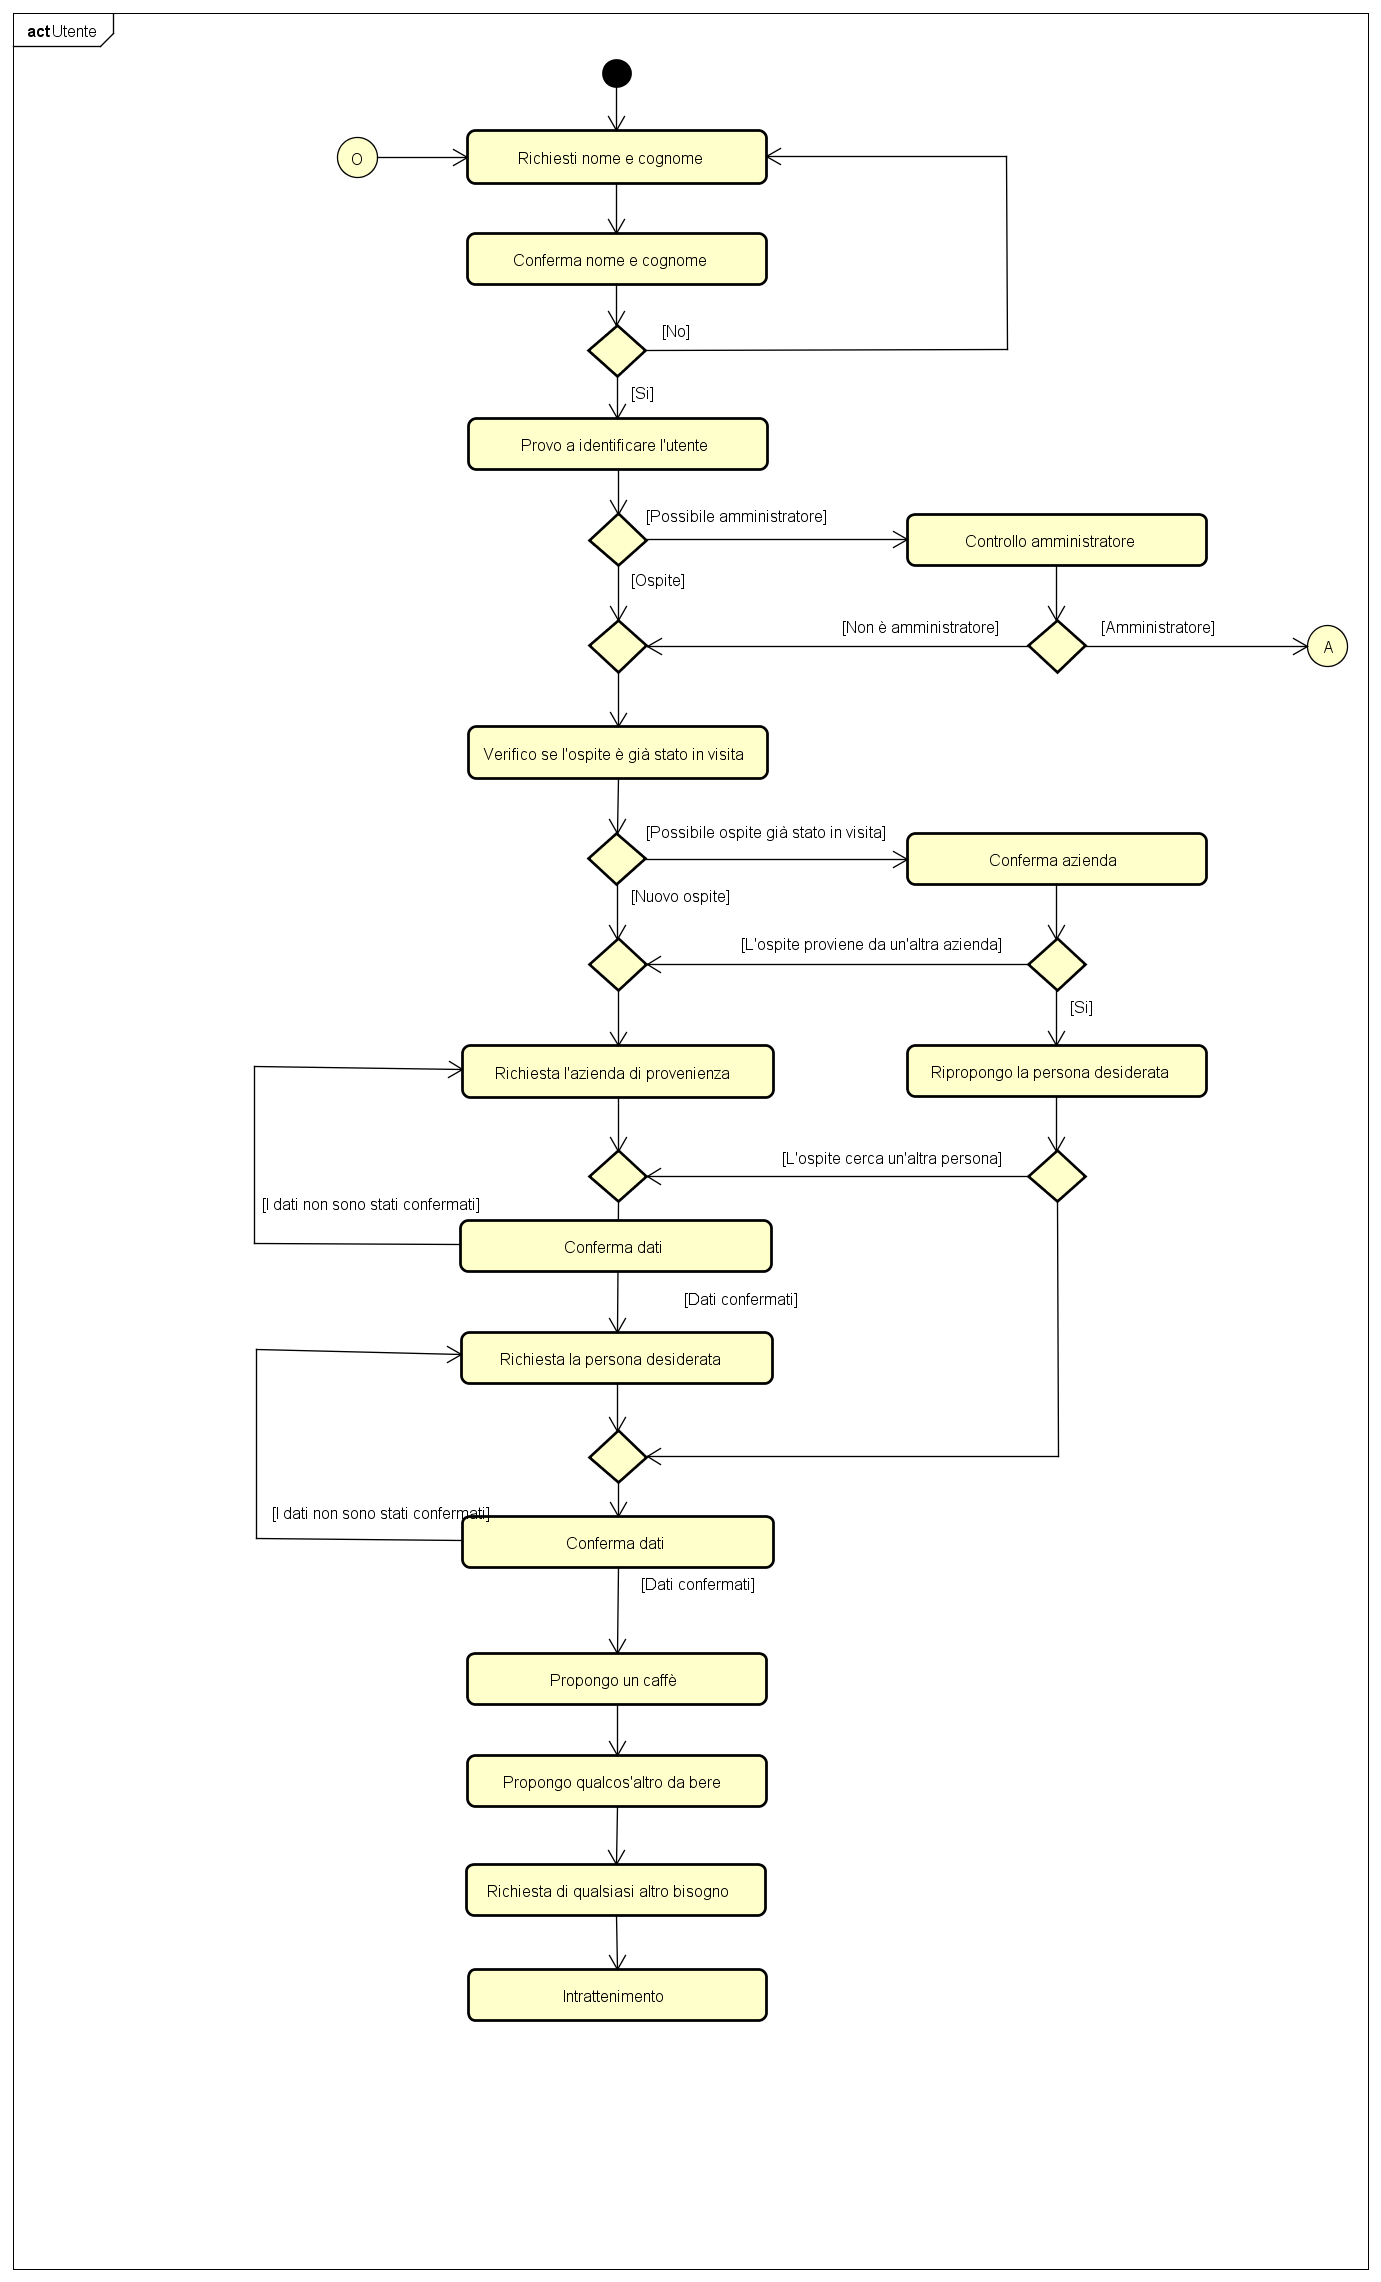
\includegraphics[width=0.7\textwidth,height=\textheight,keepaspectratio]{sezioni/images/Utente.png}}
	\caption{Flusso del dialogo per un ospite}\label{fig:flussoOspite}
\end{figure}
\newpage
\subsubsection{Amministratore}\label{admin}
Le funzionalità disponibili ad un amministratore del sistema sono le seguenti:
\begin{itemize}
	\item effettuare l'accesso all'area di amministrazione;
	\item aggiunta di una \gl{rule} (\gl{direttiva});
	\item rimozione di una rule;
	\item aggiornamento di una rule;
	\item lettura di una o più rule;
	\item aggiunta di un \gl{target};
	\item aggiornamento di un target;
	\item rimozione di un target;
	\item aggiornare i propri dati;
	\item lettura di uno o più amministratori.
\end{itemize}
\paragraph{Effettuare l'accesso all'area di amministrazione}\label{adminArea}
Solo gli utenti registrati possono effettuare l'accesso all'area di amministrazione. La registrazione di un nuovo amministratore è consentita solo al super amministratore del sistema, la quale procedura è spiegata in \ref{AddAdmin}. \\
Per effettuare l'accesso, seguire la seguente procedura:
\begin{itemize}
	\item esordire con un saluto (ad esempio "Hi", "Hello", "Good morning");
	\item \PROGETTO{} darà il benvenuto in azienda e chiederà il nome e il cognome dell'interlocutore. È importante che vengano forniti sia nome che cognome e non solo uno di essi;
	\item pronunciare nome e cognome;
	\item \PROGETTO, cercando nel database apposito, tenterà di capire se i dati forniti sono associati ad un amministratore esistente. Se sì, due scenari sono possibili:
	\begin{itemize}
		\item un solo amministratore esistente è associato ai dati forniti, \PROGETTO{} recupererà dal database l'username e chiederà conferma all'interlocutore;
		\item più amministratori sono associati ai dati forniti, \PROGETTO{} chiederà quindi che venga comunicato l'username dell'amministratore con il quale effettuare l'accesso. Successivamente, viene chiesta conferma; 
	\end{itemize}
	Altrimenti, l'interlocutore viene trattato come un ospite;
	\item se corretti, dare conferma dei dati recuperati da \PROGETTO, smentire altrimenti;
	\item pronunciare la frase di riconoscimento che \PROGETTO{} fornirà.
\end{itemize}
\paragraph{Aggiunta di una rule}
Per aggiungere una rule, seguire la seguente procedura:
\begin{itemize}
	\item pronunciare una frase del tipo "add rule" o "I want to add a rule";
	\item \PROGETTO{} chiederà di inserire un parametro per volta (nome della rule, \gl{task} e \gl{target});
	\item una volta raccolti, \PROGETTO{} chiederà la conferma dei dati;
	\item se si nega la conferma, si ritornerà al pannelo di amministrazione.
\end{itemize}
Alla voce \gl{task} nel glossario (\ref{task}) è presente l'elenco dei task supportati.
\paragraph{Rimozione di una rule}
Per rimuovere una rule, seguire la seguente procedura:
\begin{itemize}
	\item pronunciare una frase del tipo "remove rule" o "I want to remove a rule";
	\item \PROGETTO{} chiederà il nome della rule che si vuole eliminare;
	\item una volta raccolti, \PROGETTO{} chiederà la conferma dei dati;
	\item se si nega la conferma, si ritornerà al pannelo di amministrazione.
\end{itemize}
Questa operazione è possibile solo sulle rule definite dall'amministratore loggato.
\paragraph{Aggiornamento di una rule}
Per aggiornare una rule, seguire la seguente procedura:
\begin{itemize}
	\item pronunciare una frase del tipo "update rule" o "I want to update a rule";
	\item \PROGETTO{} chiederà il nome della rule che si vuole aggiornare;
	\item una volta raccolti, \PROGETTO{} chiederà la conferma dei dati;
	\item se si nega la conferma, si ritornerà al pannelo di amministrazione.
\end{itemize}
Vista la natura dell'input di tipo vocale, i \gl{target} di una rule devono essere aggiornati a parte, come spiegato in \ref{updateRuleTarget}.
Questa operazione è possibile solo sulle rule definite dall'amministratore loggato.
\paragraph{Lettura di una o più rule}
Per ottenere i dati di una rule, seguire la seguente procedura:
\begin{itemize}
	\item pronunciare una frase del tipo "get rule" o "I want to retrieve a rule";
	\item \PROGETTO{} chiederà il nome della rule che si vuole ottenere;
	\item se esistente, verrà restituita la relativa rule.
\end{itemize}

Per ottenere i dati di tutte le rule esistenti, pronunciare una frase del tipo "get all rule", "get rule list" o "retrieve all rules".
\paragraph{Aggiunta di un target}\label{addRuleTarget}
Per aggiungere un target ad una rule, seguire la seguente procedura:
\begin{itemize}
	\item pronunciare una frase del tipo "add rule target" o "I want to add a rule target";
	\item \PROGETTO{} chiederà il nome della rule nella quale aggiungere il target;
	\item \PROGETTO{} chiederà di pronunciare i parametri del nuovo target (nome, azienda di provenienza, \gl{member});
	\item una volta raccolti, \PROGETTO{} chiederà la conferma dei dati;
	\item se si nega la conferma, si ritornerà al pannelo di amministrazione.
\end{itemize}
\paragraph{Rimozione di un target}
Per rimuovere un target da una rule, seguire la seguente procedura:
\begin{itemize}
	\item pronunciare una frase del tipo "remove rule target" o "I want to remove a rule target";
	\item \PROGETTO{} chiederà il nome della rule dalla quale rimuovere il target;
	\item \PROGETTO{} chiederà di pronunciare i parametri del target da rimovere (nome, azienda di provenienza, \gl{member});
	\item una volta raccolti, \PROGETTO{} chiederà la conferma dei dati;
	\item se si nega la conferma, si ritornerà al pannelo di amministrazione.
\end{itemize}
Questa operazione è possibile solo sulle rule definite dall'amministratore loggato.
\paragraph{Aggiornamento di un target}\label{updateRuleTarget}
Per aggiornare un target di una rule, seguire la seguente procedura:
\begin{itemize}
	\item pronunciare una frase del tipo "update rule target" o "I want to update a rule target";
	\item \PROGETTO{} chiederà il nome della rule nella quale aggiornare il target;
	\item \PROGETTO{} chiederà di pronunciare i parametri del target da aggiornare (nome, azienda di provenienza, \gl{member});
	\item una volta raccolti, \PROGETTO{} chiederà la conferma dei dati;
	\item se si nega la conferma, si ritornerà al pannelo di amministrazione.
\end{itemize}
Questa operazione è possibile solo sulle rule definite dall'amministratore loggato.
\paragraph{Aggiornamento dei propri dati}

Per aggiornare i propri dati, l'amministratore loggato deve seguire la seguente procedura:
\begin{itemize}
	\item pronunciare una frase del tipo "update data" o "I want to update my data";
	\item \PROGETTO{} chiederà i nuovi dati da aggiornare;
	\item una volta raccolti, \PROGETTO{} chiederà la conferma dei dati;
	\item se si nega la conferma, si ritornerà al pannelo di amministrazione.
\end{itemize}

\paragraph{Lettura di uno o più amministratori}
Per ottenere i dati di un amministratore, seguire la seguente procedura:
\begin{itemize}
	\item pronunciare una frase del tipo "get user" o "I want to retrieve a user";
	\item \PROGETTO{} chiederà il nome dell'amministratore che si vuole ottenere;
	\item se esistente, verrà restituito il relativo amministratore (dati sensibili esclusi).
\end{itemize}

Per ottenere i dati di tutti gli amministratori esistenti (dati sensibili esclusi), pronunciare una frase del tipo "get all users", "get users list" o "I want to retrieve all users".

\subsubsection{Super Amministratore}\label{superAdmin}
Un super amministratore è un amministratore con privilegi maggiori, in quanto può operare su tutti gli utenti del sistema e le rule indipendentemente da chi le abbia create, con anche un numero di funzionalità più grande rispetto agli amministratori.
Infatti, in caso un amministratore venga eliminato dal sistema (operazione possibile solo per il super amministratore), le rule da lui create non saranno eliminate, ma saranno comunque sotto il controllo del super amministratore. \\
Le funzionalità aggiuntive sono:
\begin{itemize}
	\item aggiunta di un amministratore;
	\item aggiornamento di un amministratore;
	\item rimozione di un amministratore;
	\item aggiunta dell'enrollment di un amministratore;
	\item rimozione dell'enrollment di un amministratore.
\end{itemize}
\paragraph{Aggiunta di un amministratore}\label{AddAdmin}
Per aggiungere un amministratore, seguire la seguente procedura:
\begin{itemize}
	\item pronunciare una frase del tipo "add admin" o "I want to add an admin";
	\item \PROGETTO{} chiederà il nome e il cognome del nuovo amministratore. È importante che vengano forniti sia nome che cognome e non solo uno di essi;
	\item \PROGETTO{} chiederà l'username del nuovo amministratore;
	\item una volta raccolti, \PROGETTO{} chiederà la conferma dei dati;
	\item se si nega la conferma, si ritornerà al \gl{pannello di amministrazione}.
\end{itemize}

Vista la natura dell'input di tipo vocale, l'\gl{enrollment} di un amministratore deve essere aggiunto a parte, come spiegato in \ref{addEnrollment}.
\paragraph{Aggiornamento di un amministratore}
 Per aggiornare un amministratore, seguire la seguente procedura:
\begin{itemize}
	\item pronunciare una frase del tipo "update admin" o "I want to update an admin";
	\item \PROGETTO{} chiederà l'username dell'amministratore che si vuole aggiornare;
	\item \PROGETTO{} chiederà l'inserimento dei nuovi dati;
	\item una volta raccolti, \PROGETTO{} chiederà la conferma dei dati;
	\item se si nega la conferma, si ritornerà al pannello di amministrazione.
\end{itemize}

\paragraph{Rimozione di un amministratore}
 Per rimuovere un amministratore, seguire la seguente procedura:
\begin{itemize}
	\item pronunciare una frase del tipo "remove admin" o "I want to remove an admin";
	\item \PROGETTO{} chiederà l'username dell'amministratore che si vuole rimuovere;
	\item una volta raccolti, \PROGETTO{} chiederà la conferma dei dati;
	\item se si nega la conferma, si ritornerà al pannello di amministrazione.
\end{itemize}

Quando un amministratore viene rimosso, le rule da lui create non vengono rimosse.
\paragraph{Aggiunta dell'enrollment di un amministratore}\label{addEnrollment}

Per aggiungere un enrollment ad un amministratore, per crearne quindi l'impronta vocale, è necessario seguire la seguente procedura:
\begin{itemize}
	\item pronunciare una frase del tipo "add enrollment" o "I want to add an enrollment";
	\item \PROGETTO{} chiederà l'username dell'amministratore al quale aggiungere l'enrollment;
	\item \PROGETTO{} mostrerà una frase la quale deve essere pronunciata dall'amministratore da aggiungere \textbf{in persona}; 
	\item una volta raccolti, \PROGETTO{} chiederà la conferma dei dati;
	\item se si nega la conferma, si ritornerà al pannello di amministrazione.
\end{itemize}
\paragraph{Reset dell'enrollment di un amministratore}

Per resettare l'enrollment di un amministratore, è necessario seguire la seguente procedura:
\begin{itemize}
	\item pronunciare una frase del tipo "reset enrollment" o "I want to reset an enrollment";
	\item \PROGETTO{} chiederà l'username dell'amministratore al quale resettare l'enrollment;
	\item una volta raccolti, \PROGETTO{} chiederà la conferma dei dati;
	\item se si nega la conferma, si ritornerà al pannello di amministrazione.
\end{itemize}